\documentclass{article}

\usepackage{hyperref}
\usepackage{fancyhdr}
\usepackage{graphicx}
\usepackage{subfigure}
\usepackage{listings}
\usepackage{setspace}
\usepackage{mathtools} % For drcases
\usepackage{amsmath, amsfonts}
\usepackage{enumerate}
\usepackage{graphicx}
\usepackage{titling}
\usepackage{algorithm}
\usepackage{algorithmicx}
\doublespacing


\newcommand{\vc}[1]{\boldsymbol{#1}}
\newcommand{\adj}[1]{\frac{d J}{d #1}}
\newcommand{\chain}[2]{\adj{#2} = \adj{#1}\frac{d #1}{d #2}}

\newcommand{\R}{\mathbb{R}}
\newcommand{\blackcircle}{\tikz\draw[black,fill=black] (0,0) circle (1ex);}
\renewcommand{\circle}{\tikz\draw[black] (0,0) circle (1ex);}

\newcommand{\emptysquare}{{\LARGE $\square$}\ \ }
\newcommand{\filledsquare}{{\LARGE $\blacksquare$}\ \ }
\newcommand{\emptycircle}{{\LARGE $\fullmoon$}\ \ }
\newcommand{\filledcircle}{{\LARGE $\newmoon$}\ \ }

\newcommand{\ntset}{test}

% mathcal
\newcommand{\Ac}{\mathcal{A}}
\newcommand{\Bc}{\mathcal{B}}
\newcommand{\Cc}{\mathcal{C}}
\newcommand{\Dc}{\mathcal{D}}
\newcommand{\Ec}{\mathcal{E}}
\newcommand{\Fc}{\mathcal{F}}
\newcommand{\Gc}{\mathcal{G}}
\newcommand{\Hc}{\mathcal{H}}
\newcommand{\Ic}{\mathcal{I}}
\newcommand{\Jc}{\mathcal{J}}
\newcommand{\Kc}{\mathcal{K}}
\newcommand{\Lc}{\mathcal{L}}
\newcommand{\Mc}{\mathcal{M}}
\newcommand{\Nc}{\mathcal{N}}
\newcommand{\Oc}{\mathcal{O}}
\newcommand{\Pc}{\mathcal{P}}
\newcommand{\Qc}{\mathcal{Q}}
\newcommand{\Rc}{\mathcal{R}}
\newcommand{\Sc}{\mathcal{S}}
\newcommand{\Tc}{\mathcal{T}}
\newcommand{\Uc}{\mathcal{U}}
\newcommand{\Vc}{\mathcal{V}}
\newcommand{\Wc}{\mathcal{W}}
\newcommand{\Xc}{\mathcal{X}}
\newcommand{\Yc}{\mathcal{Y}}
\newcommand{\Zc}{\mathcal{Z}}

% mathbb
\newcommand{\Ab}{\mathbb{A}}
\newcommand{\Bb}{\mathbb{B}}
\newcommand{\Cb}{\mathbb{C}}
\newcommand{\Db}{\mathbb{D}}
\newcommand{\Eb}{\mathbb{E}}
\newcommand{\Fb}{\mathbb{F}}
\newcommand{\Gb}{\mathbb{G}}
\newcommand{\Hb}{\mathbb{H}}
\newcommand{\Ib}{\mathbb{I}}
\newcommand{\Jb}{\mathbb{J}}
\newcommand{\Kb}{\mathbb{K}}
\newcommand{\Lb}{\mathbb{L}}
\newcommand{\Mb}{\mathbb{M}}
\newcommand{\Nb}{\mathbb{N}}
\newcommand{\Ob}{\mathbb{O}}
\newcommand{\Pb}{\mathbb{P}}
\newcommand{\Qb}{\mathbb{Q}}
\newcommand{\Rb}{\mathbb{R}}
\newcommand{\Sb}{\mathbb{S}}
\newcommand{\Tb}{\mathbb{T}}
\newcommand{\Ub}{\mathbb{U}}
\newcommand{\Vb}{\mathbb{V}}
\newcommand{\Wb}{\mathbb{W}}
\newcommand{\Xb}{\mathbb{X}}
\newcommand{\Yb}{\mathbb{Y}}
\newcommand{\Zb}{\mathbb{Z}}

% mathbf lowercase
\newcommand{\av}{\mathbf{a}}
\newcommand{\bv}{\mathbf{b}}
\newcommand{\cv}{\mathbf{c}}
\newcommand{\dv}{\mathbf{d}}
\newcommand{\ev}{\mathbf{e}}
\newcommand{\fv}{\mathbf{f}}
\newcommand{\gv}{\mathbf{g}}
\newcommand{\hv}{\mathbf{h}}
\newcommand{\iv}{\mathbf{i}}
\newcommand{\jv}{\mathbf{j}}
\newcommand{\kv}{\mathbf{k}}
\newcommand{\lv}{\mathbf{l}}
\newcommand{\mv}{\mathbf{m}}
\newcommand{\nv}{\mathbf{n}}
\newcommand{\ov}{\mathbf{o}}
\newcommand{\pv}{\mathbf{p}}
\newcommand{\qv}{\mathbf{q}}
\newcommand{\rv}{\mathbf{r}}
\newcommand{\sv}{\mathbf{s}}
\newcommand{\tv}{\mathbf{t}}
\newcommand{\uv}{\mathbf{u}}
\newcommand{\vv}{\mathbf{v}}
\newcommand{\wv}{\mathbf{w}}
\newcommand{\xv}{\mathbf{x}}
\newcommand{\yv}{\mathbf{y}}
\newcommand{\zv}{\mathbf{z}}

% mathbf uppercase
\newcommand{\Av}{\mathbf{A}}
\newcommand{\Bv}{\mathbf{B}}
\newcommand{\Cv}{\mathbf{C}}
\newcommand{\Dv}{\mathbf{D}}
\newcommand{\Ev}{\mathbf{E}}
\newcommand{\Fv}{\mathbf{F}}
\newcommand{\Gv}{\mathbf{G}}
\newcommand{\Hv}{\mathbf{H}}
\newcommand{\Iv}{\mathbf{I}}
\newcommand{\Jv}{\mathbf{J}}
\newcommand{\Kv}{\mathbf{K}}
\newcommand{\Lv}{\mathbf{L}}
\newcommand{\Mv}{\mathbf{M}}
\newcommand{\Nv}{\mathbf{N}}
\newcommand{\Ov}{\mathbf{O}}
\newcommand{\Pv}{\mathbf{P}}
\newcommand{\Qv}{\mathbf{Q}}
\newcommand{\Rv}{\mathbf{R}}
\newcommand{\Sv}{\mathbf{S}}
\newcommand{\Tv}{\mathbf{T}}
\newcommand{\Uv}{\mathbf{U}}
\newcommand{\Vv}{\mathbf{V}}
\newcommand{\Wv}{\mathbf{W}}
\newcommand{\Xv}{\mathbf{X}}
\newcommand{\Yv}{\mathbf{Y}}
\newcommand{\Zv}{\mathbf{Z}}

% bold greek lowercase
\newcommand{\alphav     }{\boldsymbol \alpha     }
\newcommand{\betav      }{\boldsymbol \beta      }
\newcommand{\gammav     }{\boldsymbol \gamma     }
\newcommand{\deltav     }{\boldsymbol \delta     }
\newcommand{\epsilonv   }{\boldsymbol \epsilon   }
\newcommand{\varepsilonv}{\boldsymbol \varepsilon}
\newcommand{\zetav      }{\boldsymbol \zeta      }
\newcommand{\etav       }{\boldsymbol \eta       }
\newcommand{\thetav     }{\boldsymbol \theta     }
\newcommand{\varthetav  }{\boldsymbol \vartheta  }
\newcommand{\iotav      }{\boldsymbol \iota      }
\newcommand{\kappav     }{\boldsymbol \kappa     }
\newcommand{\varkappav  }{\boldsymbol \varkappa  }
\newcommand{\lambdav    }{\boldsymbol \lambda    }
\newcommand{\muv        }{\boldsymbol \mu        }
\newcommand{\nuv        }{\boldsymbol \nu        }
\newcommand{\xiv        }{\boldsymbol \xi        }
\newcommand{\omicronv   }{\boldsymbol \omicron   }
\newcommand{\piv        }{\boldsymbol \pi        }
\newcommand{\varpiv     }{\boldsymbol \varpi     }
\newcommand{\rhov       }{\boldsymbol \rho       }
\newcommand{\varrhov    }{\boldsymbol \varrho    }
\newcommand{\sigmav     }{\boldsymbol \sigma     }
\newcommand{\varsigmav  }{\boldsymbol \varsigma  }
\newcommand{\tauv       }{\boldsymbol \tau       }
\newcommand{\upsilonv   }{\boldsymbol \upsilon   }
\newcommand{\phiv       }{\boldsymbol \phi       }
\newcommand{\varphiv    }{\boldsymbol \varphi    }
\newcommand{\chiv       }{\boldsymbol \chi       }
\newcommand{\psiv       }{\boldsymbol \psi       }
\newcommand{\omegav     }{\boldsymbol \omega     }

% bold greek uppercase
\newcommand{\Gammav     }{\boldsymbol \Gamma     }
\newcommand{\Deltav     }{\boldsymbol \Delta     }
\newcommand{\Thetav     }{\boldsymbol \Theta     }
\newcommand{\Lambdav    }{\boldsymbol \Lambda    }
\newcommand{\Xiv        }{\boldsymbol \Xi        }
\newcommand{\Piv        }{\boldsymbol \Pi        }
\newcommand{\Sigmav     }{\boldsymbol \Sigma     }
\newcommand{\Upsilonv   }{\boldsymbol \Upsilon   }
\newcommand{\Phiv       }{\boldsymbol \Phi       }
\newcommand{\Psiv       }{\boldsymbol \Psi       }
\newcommand{\Omegav     }{\boldsymbol \Omega     }



%\lhead{\includegraphics[width=0.2\textwidth]{nyush-logo.pdf}}
\fancypagestyle{firstpage}{%
  \lhead{15-418/15-618: Parallel Computer Architecture and Programmin}
  \rhead{
   Alicia Luo, Chuyi Zhang}
}

\RequirePackage[
	left=1.5in,
	right=1.5in,
	top=1in,
	bottom=1in,
]{geometry}

%%%% PROJECT TITLE
\title{Final Project Report\\
        \Large \emph{A GPU-based Parallel Training System with Parameter Server and Explicit Memory Management}}

%%%% NAMES OF ALL THE STUDENTS INVOLVED (first-name last-name)
\author{\href{mailto:tingluo@andrew.cmu.edu}{Alicia Luo(tingluo@andrew.cmu.edu)} \href{mailto:tingluo@andrew.cmu.edu}{Chuyi Zhang(chuyiz@andrew.cmu.edu)}}


\date{\vspace{-5ex}} %NO DATE


\begin{document}
\maketitle
\thispagestyle{firstpage}
\section*{SUMMARY}
% A short (no more than a paragraph) project summary. If applicable, the summary should list your project deliverables (including what you plan to show at the parallelism competition) and what machines they ran on. 

We implemented a GPU-based logistic regression training system with a parameter server and an explicit memory management policy, mainly based on the system design presented by "GeePS: Scalable Deep Learning on Distributed GPUs with a GPU-specialized Parameter Server" [1], which we will refer to as "the paper". Our training system can run large parameter models that are normally restricted by limited GPU memory. When the allocated GPU memory is not large enough to hold all the training data and model parameters, the worker nodes will actively move data between CPU and GPU through a heuristic data placement policy. Our implementation is capable of optimizing the training efficiency by pinning part of model parameters and training data in the GPU memory to reduce the amount of data movement. We also added support for configurable parameters to dedicate GPU memory space to the access buffer pool, the pinned dataset, and the pinned parameter cache as the user wishes. Finally, our system is scalable in dataset size with the collaboration between worker nodes through a parameter server.

\section*{BACKGROUND}
\subsection*{Logistic Regression Algorithm}
Logistic regression is a powerful machine learning algorithm to solve classification problems. It accepts a set of model parameters (denoted as $\xv$), multiplies with corresponding weights (denoted as $\thetav$), passes through the sigmoid function ($\frac{1}{1+\exp{-x}}$), and finally produce a probability ($\pv$) between $0$ and $1$. A prediction of $\hat{y} = 1$ will be made when $\pv(\xv) >= 0.5$ and $\hat{y} = 0$ otherwise.

$$
p_\thetav(y = 1 |\xv) = \frac{1}{1+\exp^{(-\thetav^T \Xv)}}$$

The loss function we will optimize is given by

\begin{align}
    J(\thetav)= - \frac{1}{N} \log p\left(\yv \mid \mathbf{X},\thetav\right) &= \frac{1}{N}\sum_{i=1}^N \left[sigmoid(\thetav^T\xv^{\left(i\right)})^{y^{(i)}}(1 - sigmoid(\thetav^T\xv^{\left(i\right)}))^{1-y^{(i)}}]
\end{align}





The partial derivative of $J(\thetav)$ with respect to $\theta_j \,, j\in\{0,...,M\}$ is:
\begin{align}
    \frac{\partial J(\thetav)}{\partial \theta_j} &= \frac{1}{N} \sum_{i=1}^N \underbrace{\left[-x_j^{\left(i\right)}\left(y^{(i)}-sigmoid(\thetav^T\xv^{\left(i\right)})\right)\right]}_{\textstyle\frac{\partial J^{(i)}(\thetav)}{\partial \theta_j}}
\end{align}


The gradient descent update rule  for binary logistic regression for parameter element $\theta_j$ is:
\begin{align}
    \theta_j \leftarrow \theta_j - \alpha \frac{\partial J(\thetav)}{\partial \theta_j}
\end{align}


Therefore, the stochastic gradient descent that the system will perform on $\theta_j$ using the $i$-th datapoint $(\xv^{(i)},y^{(i)})$ is given by the below update rule:

\begin{align}
    \theta_j \leftarrow \theta_j + \alpha x_j^{\left(i\right)} \left[y^{(i)}-sigmoid(\thetav^T\xv^{\left(i\right)})\right]
\end{align}
 
\subsection*{Working with Sparse Dataset}
Since we are working on a very large dataset with huge number of parameters, the data samples are stored in a sparse format to avoid unnecessary memory consumption. The feature information of each sample is stored as two arrays: the feature ID array and the feature value array. In our sequential C++ CPU implementation, data samples are represented with the following structure:
\begin{figure}[htp]
    \centering
    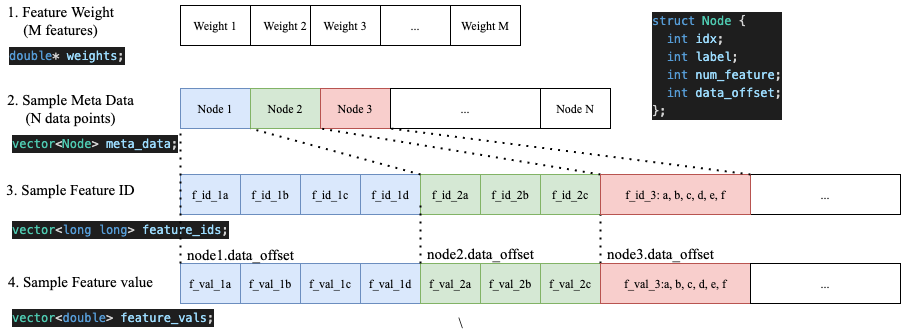
\includegraphics[width=14cm]{cpu_data_structure.png}
    \caption{Key data structures in sequential CPU implementation}
\end{figure}



\subsection*{Workflow Breakdown and Benefit of Parallelization}

Because our dataset is composed of tens of thousands of features and millions of samples, a simple CPU approach would be slow to solve problems at this scale. Instead, we took the data-parallel approach to process the data samples on a distributed set of worker nodes, utilize SIMD operations on GPU to boost up the highly parallelable workloads, and manage CPU/GPU memory explicitly to enable large model training and improve performance.

\textbf{Computation Dependency}: The logistic regression algorithm will iterate over all data points. For each individual point, it multiplies feature values with corresponding weights and predicts the label after a sigmoid transformation. According to our loss function mentioned above, the major update rule for weights is given by the expression 3:
$$
    \theta_j \leftarrow \theta_j + \alpha x_j^{\left(i\right)} \left[y^{(i)}-sigmoid(\thetav^T\xv^{\left(i\right)})\right]
$$
Between two updates, there is a dependency on the weights that the two different data points are multiplying with. Because stochastic gradient descent algorithm is insensitive to data staleness, we decided to relax the model consistency to batch level and perform synchronization on parameters after each batch.


\textbf{Data Parallel}: Because the logistic regression algorithm only involves one multiplication and one transformation, there is not enough room for model parallelism. With the dependency analysis above and the relaxation of model consistency on weights, we are able to adopt a data parallel approach to accelerate the training procedure of our system. Since an identical function consisting of multiplication and transformation is applied to all data samples of each batch independently, we decided to leverage GPU and SPMD programming. Parameter server implemented through MPI on multiple nodes can further enlarge the scale of data parallel.


\subsection*{Challenges of Limited GPU Memory}
GPU acceleration has been a common approach to offload the computation-intensive portion of the program from CPU by taking advantage of parallelism. Although GPUs devote more transistors to compute data processing, there is a limitation on the size of model parameters that a GPU-accelerated program could support. Taking PSC Bridges-2 as an example, the RAM size of a regular node is 256 GB, which means a CPU-based training system can hold a model with a size up to 256 GB. However, the memory size of a V100 GPU is 16 GB. Since GPU requires a complete set of model parameters to run an inference or conduct a forward computation of a training process, a GPU-based acceleration approach only works for models that can fit into the GPU memory. Such memory restriction largely limits the size of model that a GPU can train and infer.

\section*{APPROACH}
\subsection*{Overview}

We would like to discuss how we implemented our highly-scalable parallel training system in several steps. To speed up the training process, our system utilizes GPU parallelism using CUDA programming in a data-parallel manner. To address the cases where datasets or models are too large to fit into GPU memory, our system takes two approaches simultaneously: parallelized batch data processing and explicit memory management. Finally, to further scale the training of large datasets, we implemented a parameter server by OpenMPI to enable collaboration between worker nodes, and it successfully fits into our GPU-based design.

\subsection*{From CPU to GPU(CUDA)}

GPU intrinsically supports SPMD operations and therefore provides strong computing capability for parallelizable jobs. However, GPUs are not suitable for general workloads like network communication. The downsides of GPU include the need to constantly transfer data between CPU and GPU because of the need to perform general operations or simply because the GPU device memory is limited.

We initially took the naive approach of porting the logistic regression algorithm with a small dataset from CPU to GPU: First, we allocate enough space on GPU memory for training data and feature weights. Second, we copy all training data samples from CPU to GPU. Third, we call the device function once for each epoch. In the GPU device function, each GPU thread process one data sample, which is independent of each other. Since there is no hard requirement on the synchronization of logistic regression within an epoch, the GPU threads perform atomic updates to the weights on GPU.

Under this approach, both the data samples and the feature weights are not transferred back to the CPU until the very end and thereby reducing unnecessary data movements. 

One obvious problem of the above approach is that it does not allow the case where the data samples or the feature weights cannot fit into the GPU device memory. We address this problem in two steps that are discussed in the following sections. 

\subsection*{Parallelized Batch Processing}

The first case that we dealt with is when the data size exceeds GPU memory. Basically, we adopted the approach of batch processing. After calculating the available space for data samples on GPU, we repeatedly send data samples in batches to GPU within each epoch. Since the dataset is sparse and the data sample size is not uniform, we perform a dynamic fitting process to put as much data sample as the memory allows in a batch.

After examining the results, we are not surprised to find out that the extra communication cost impairs the performance. GPU's computation on each batch depends on the arrival of the batch data. It would be a waste in time and computing power to let GPU wait for the batch data while doing nothing. A better approach, as suggested in the paper, is to perform data transfer in the background and thereby hide the latency. Specifically, we divided the available space for data on GPU into two, representing the foreground data samples and background data samples correspondingly. We then overlap the background data transfer with the kernel function that performs on the foreground data to keep GPU busy.

\subsection*{Memory Management}

Another important case to address is the size of parameters in the model. If GPU memory is not enough to store all the feature weights, one solution is to utilize the memory on the CPU. For each batch of data sent to GPU, we can analyze the relevant features and sends these needed feature weights along. As mentioned in the paper, it is also possible to pin a portion of parameters on GPU as in Figure 2, so that the read and update operations of this portion are only performed on GPU. By doing so, for each data sample transmitted, the size of relevant feature weights that are sent along can be reduced. Therefore the communication overhead gets lower. Figure 3 includes the detailed data structures to realize the communication between CPU and GPU under the setting of data batch processing and partially pinned parameters discussed above.

\begin{figure}[htp]
    \centering
    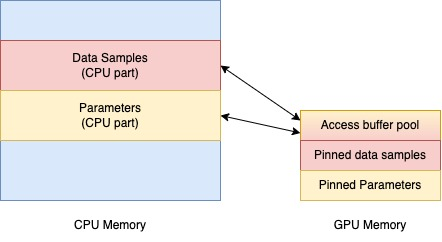
\includegraphics[width=8cm]{memory_management_1.jpg}
    \caption{Key memory allocations on CPU and GPU (single node)}
\end{figure}

Similarly, data samples can be partially pinned on GPU, as shown in Figure 2. The benefits of this approach also include reducing communication when data samples cannot totally fit into GPU memory. Under this approach, only the unpinned portion needs to be transmitted in batches. There is a balance to be reached in choosing the access buffer size and the pinned data size. 

To conclude, the current memory management model is illustrated in Figure 2. Assuming the system is set up with partially pinned data samples and parameters, the CPU memory contains the unpinned portion of data samples and parameter weights. The GPU memory is divided into an allocated space for pinned data samples, an allocated space for pinned parameters, and an access buffer pool that exchanges both data samples and parameter weights with CPU. For data samples, the uni-direction data transmission from CPU to GPU occurs in every batch. For parameter weights, the data exchange is bi-directional, which includes reads and updates. 

Our system allows the user to configure the sizes of the different dedicated spaces on GPU. The detailed algorithm is shown below:

\begin{figure}[htp]
    \centering
    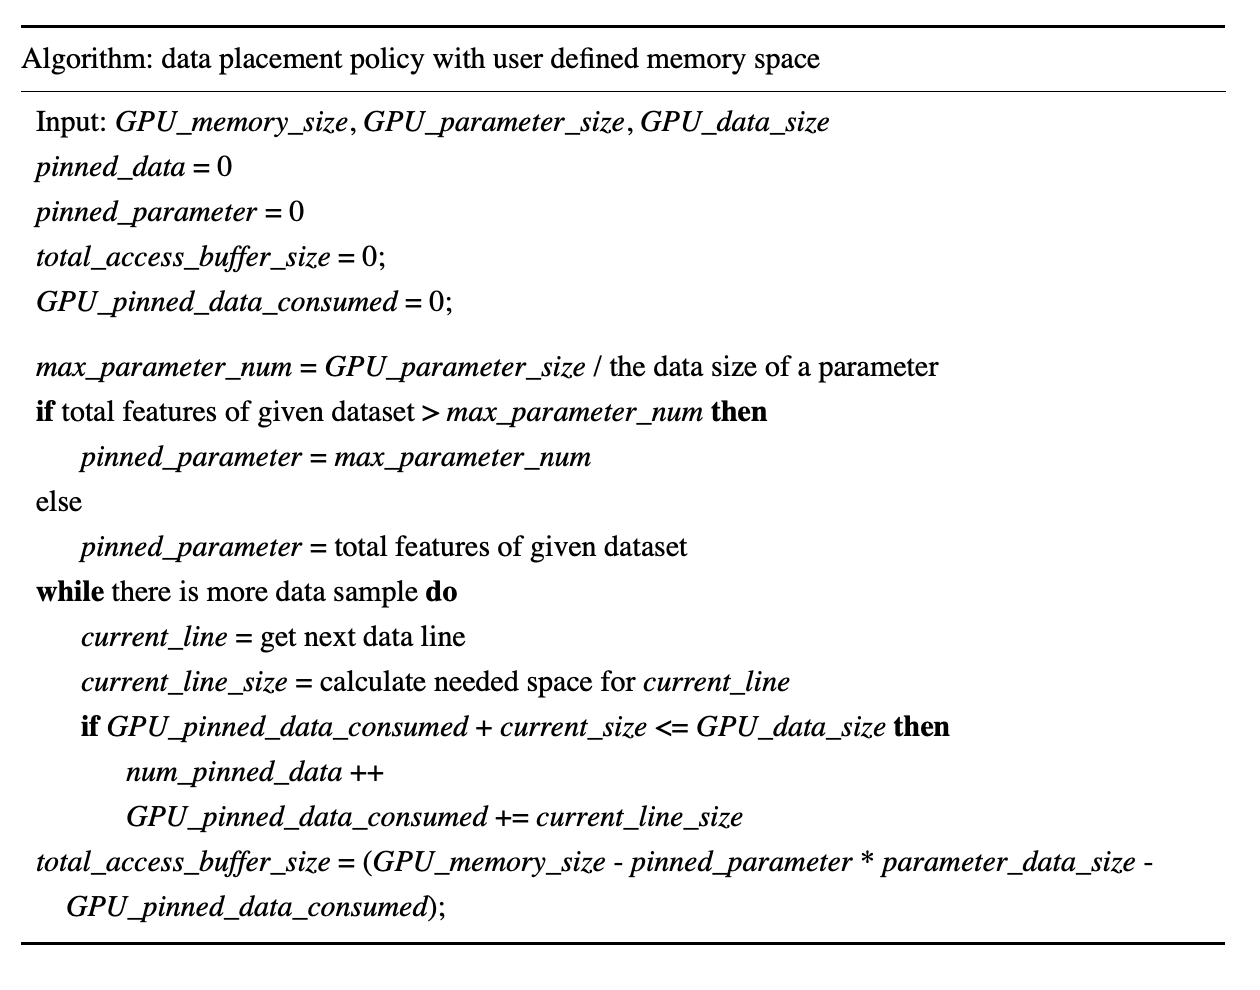
\includegraphics[width=14cm]{memory_management_policy.png}
\end{figure}

\subsection*{Parameter Server}

To scale the training of large datasets and gain performance by exploiting resources on multiple nodes, using a parameter server to serve the parameter model is a common choice. We integrated the parameter server into our approach through our message-passing protocol built by OpenMPI. Due to limitations in time and GPU resources, we chose to simulate the cluster environment using Pthread. The current memory structure is shown below in Figure 3.

\begin{figure}[htp]
    \centering
    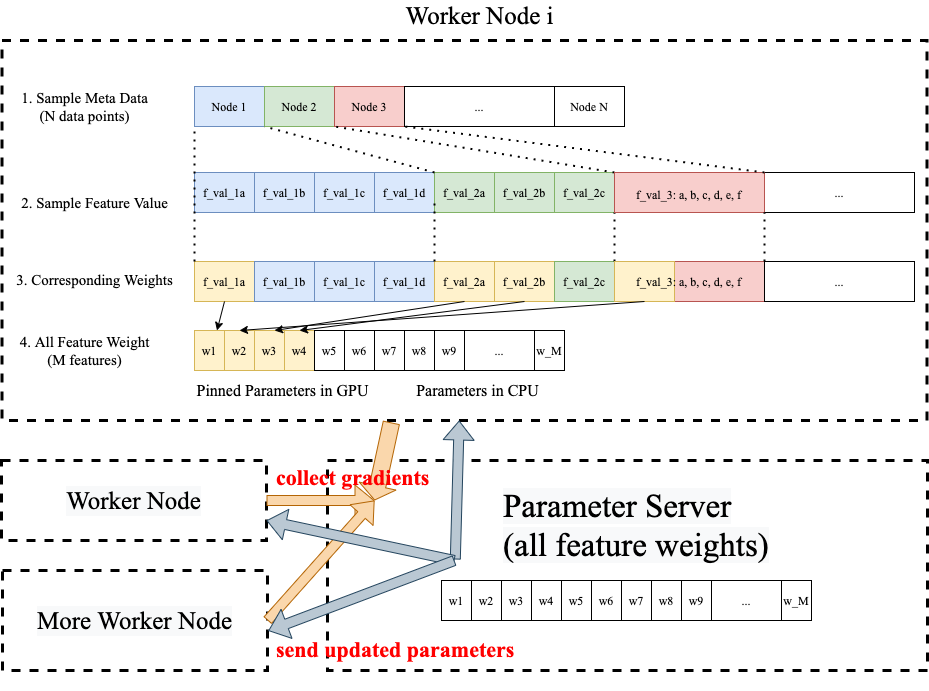
\includegraphics[width=14cm]{parameter_server.png}
    \caption{Parameter update after each batch}
\end{figure}

The cluster includes a server node and several worker nodes. In each epoch, the server broadcasts the feature weights to all workers. The workers maintain a copy of the feature weights in the CPU, transmit the pinned portion of feature weights to GPU and then perform the training process as before. After the training is done, the workers get gradients by coping the updated pinned weights on GPU back to CPU and subtracting between the updated weights and the original ones. The server then reduce the gradients and performs updates on feature weights accordingly. 

\section*{Results}
\subsection*{Configuration and Dataset Overview}
We conducted our experiments using GHC machines with NVIDIA GeForce RTX 2080 B GPUs (8 GB memory size). The dataset is KDD2010, which is composed of 8,407,752 samples and 20,216,830 features. The learning rate is 0.00001 and we will train for 10 epochs.

\subsection*{Naive CUDA Implementation}
Supposing we are in an experimental setting where the GPU is large enough to hold all the model parameters, then we can place all parameters inside GPU. In this case, there is no data movement on model parameters between GPU and CPU.

\begin{table}[!ht]
    \centering
    \begin{tabular}{|l|l|l|l|}
    \hline
        \ & CPU & GPU (No data cached) & GPU (All data cached) \\ \hline
        \# params in CPU & 20,216,830  & 0 & 0  \\ \hline
        \# params pinned in GPU & \ & 20,216,830 & 20,216,830  \\ \hline
        \# data in CPU & 305,613,510 & 305,613,510 & 0  \\ \hline
        \# data pinned in GPU & \ & 0 & 305,613,510  \\ \hline
        Training time (10 epoch) & 31.61s & 7.65s & 2.78s  \\ \hline
    \end{tabular}
\end{table}

Compared with the baseline sequential CPU implementation, both GPU versions demonstrate a significant performance gain over the sequential CPU implementation. They achieve this speedup by parallelizing the forward and backward computation of each sample point.

Although the GPU memory size might be able to hold all model parameters, it may not be able to store all data samples. We address this problem by feeding data samples from CPU to GPU in batches. Because of data locality, the all data cached GPU version is faster than no data cached GPU version. But both GPU versions achieve significant performance gain over the sequential CPU implementation.

Because we use \quoteatomic{atomic\_add} to update the model parameters pinned in GPU memory, this largely limits the optimal speedup we can achieve with CUDA.

\subsection*{Explicit Memory Management}
Since the limited GPU memory size has become a great challenge for machine learning training with a large model size, we proposed an explicit memory management policy to address this memory constraint. By varying the size of GPU memory that is allocated to the program, we can imitate the scenario where the GPU size is not able to hold all model parameters. We increased the amount the GPU memory allocated for each experiment and fixed the percentage of memory that is used to cache model parameters. The table below indicates the number and percentage of model parameters each program is able to store as a result of different GPU sizes.

\begin{table}[!ht]
    \centering
    \begin{tabular}{|l|l|l|l|l|l|}
    \hline
        \ & 1 & 2 & 3 & 4 & 5 \\ \hline
        \# params pinned in GPU & 1,342,177& 4,026,531 & 8,053,063 & 16,106,127 &20,216,830  \\ \hline
        \% params pinned in GPU & 6.6\% & 19.9\% & 39.8\% & 79.6 \% &100\%  \\ \hline
        Training time (10 epoch) & 11.44s &  10.13s & 9.44s & 8.20s & 7.52s  \\ \hline
    \end{tabular}
\end{table}

The training time decreases as the percentage of parameters being cached increases. This negative relationship is a result of data locality. When more model parameters are cached, there is less data movement between CPU and GPU during each batch of training. This table also indicates that almost 50\% time will be spent on data movement if there is no caching.

\subsection*{Parameter Server Implementation}

Our parameter server implementation further scales the logistic regression training process. The simulated cluster contains three worker nodes, each with 2GB GPU device memory, and one acting as the parameter server. The following result is a comparison between the training time of running our dataset on a single node and the cluster with the parameter server.


\begin{table}[!ht]
    \centering
    \begin{tabular}{|l|l|l|}
    \hline
        \ & Single Node & Parameter Server (3 nodes) \\ \hline
        \ All params pinned in GPU & 7.52s &  2.67s \\ \hline
        \ None params pinned in GPU & 13.54s &  7.77s \\ \hline
    \end{tabular}
\end{table}

As can be seen from the table, the cluster with a parameter server significantly speeds up the training in both cases regardless of whether the parameters are pinned in GPU or not. Possible limitations of the speedup include the extra communication cost produced by the transfer of parameter reads and updates between server and workers in each epoch. Even the pinned parameters, which stay in the GPU memory through the training process in the single node setting, need to be collected for global updates. Therefore, it would be more reasonable to favor data pinning over parameter pinning in the GPU.


\section*{Reference}
[1] Henggang Cui, Hao Zhang, Gregory R. Ganger, Phillip B. Gibbons, and Eric P. Xing. 2016. GeePS: scalable deep learning on distributed GPUs with a GPU-specialized parameter server. In Proceedings of the Eleventh European Conference on Computer Systems (EuroSys '16). Association for Computing Machinery, New York, NY, USA, Article 4, 1–16. DOI:https://doi.org/10.1145/2901318.2901323

\noindent[2] https://docs.nvidia.com/cuda/cuda-c-programming-guide/index.html

\noindent[3] https://ml-cheatsheet.readthedocs.io/en/latest/logistic_regression.html

\noindent[4] 10-301 + 10-601, Spring 2022: Introduction to Machine Learning. http://www.cs.cmu.edu/~mgormley/courses/10601/coursework.html


\section*{Distribution of Work}
Our distribution of work is quite even. We almost completed all procedures together, including literature research, framework design, and program implementation. We have a very good practice of pair programming, which prevented us from making careless mistakes and helped us write high-quality codes.


\end{document}
